\chapter{Event Vertex Reconstruction}
\label{chPositionReconstruction}

%\section{Reconstruction of the XY Coordinates}
%\label{secXYreconstruction}

A large fraction of the proportional scintillation signal (S2), produced by the collision of the extracted electrons with the xenon atoms in the gas phase, is detected by the 98 PMTs of the top array (see Section~\ref{secLCEs2}). Due to the homogeneous electric field in the target volume, and a small dispersion of the electron cloud in liquid xenon, the secondary scintillation pulse has almost the same $XY$ coordinates as the particle interaction site. The relatively small size of the PMTs used in the XENON100 detector (one square inch) provides a granularity, which is good enough to reconstruct the position of events with a millimeter resolution based on the relative number of photoelectrons collected by each of the PMTs.

Together with the $Z$-coordinate, which is inferred from the time delay between the prompt S1 and the delayed S2 signal (see Fig.~\ref{figWaveform}) and a known electron drift velocity, this provides the possibility to reconstruct the position of an event in 3D space, hence to fiducialize the liquid xenon target, and to reject multiple scattering interactions.

Three different algorithms have been used in XENON100 to reconstruct the $XY$ vertex of the interactions, based on $\chi^{2}$-minimization \cite{Yuan}, support vector machine regression (SVM) \cite{Antonio} and a  neural network (NN). The latter, which has been developed in the framework of this thesis, has the fastest performance in the data processing, and provides better position resolution than the other two methods.


\section{Neural Networks Method}
\label{secNN}

\begin{floatingfigure}[r]{0.4\textwidth}
%\begin{figure}[!h]
\centering
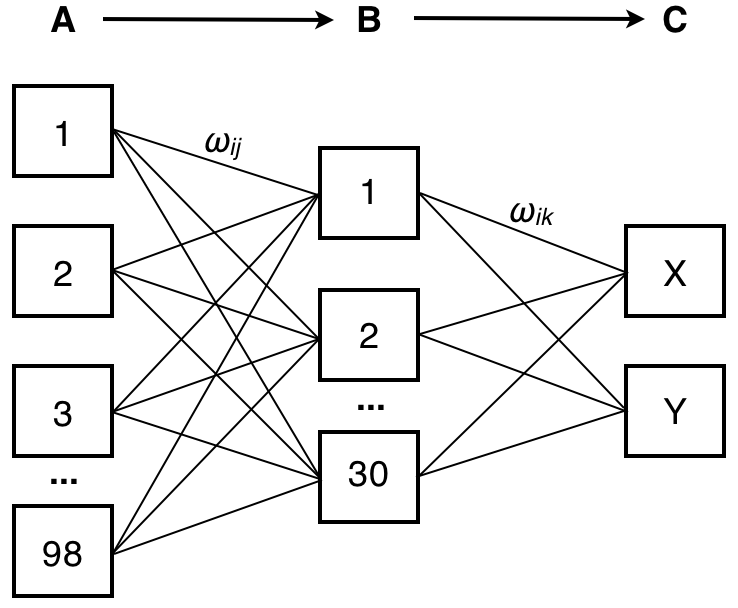
\includegraphics[width=0.4\linewidth]{plots/NN/NNscheme_withWeightsAndArrows.png}
\caption[Architecture of the two-layer perceptron used for the NN reconstruction algorithm in XENON100]{Architecture of the two-layer perceptron used for the NN reconstruction algorithm in XENON100: A - input layer, B - hidden layer, C - output layer; $\omega$ - links between neurons.}
\label{figNNscheme}
%\end{figure}
\end{floatingfigure}

Artificial neural networks (NN) are widely used for pattern recognition~\cite{PatternRecognition}. A NN consists of units and directed, weighted links between them~(Fig.~\ref{figNNscheme}). Each unit receives a net input that is computed from the weighted outputs of prior units with connections leading to this unit. Then, the new `activation' from this net input is computed, and the output function takes this result to generate the output of the unit. When the entire network has been executed, the outputs of the output layer act as the output of the entire network. 

The NN algorithm has been developed for the XENON100 experiment with the Stuttgart Neural Network Simulator (SNNS) software~\cite{SNNS}, which consists of a system kernel (version 4.3), batch simulator, and a C network compiler. The networks can be created with a Java graphical user interface, which gives a graphical representation of the NN and controls the kernel during the simulation run.

For the current application, the NN has been created as a two-layer perceptron~\cite{Perceptron} with 98 input layers representing the top PMT array, one hidden layer with 30 neurons in them, and two output neurons providing the {\it X} and {\it Y} coordinates of an event (Fig.~\ref{figNNscheme}). The optimal configuration of the hidden layer has been found empirically. The value of each neuron depends only on the neurons of the previous layer, thus the network is feed-forward.

The essential part of the algorithms based on NN is that they have to be trained on a dataset, for which the output is known for each configuration of the input parameters. The XENON100 NN algorithm has been trained on Monte Carlo data. The modeling of S2 signal and photon propagation has been performed with GEANT4 as described in Section~\ref{secLCEs2}, an example of the simulated light pattern is shown in Fig.~\ref{figLightPattern}. The patterns have been normalized by the total number of photons detected by all PMTs of the top array. 
The training dataset contains 180'000 events, uniformly distributed in $XY$ plane\footnote{The SVM and $\chi^{2}$ have been trained on a dataset with events distributed within a lattice.}. between the gate and anode meshes within a 1~mm thick layer of LXe. This corresponds to the density of 2.5 events/mm$^{2}$. In each point 3'000 optical photons have been isotropically emitted. 
The algorithm has been trained with a backpropagation learning algorithm, in which the weights between the units are adjusted with a generalized delta-rule~\cite{DeltaRule}:

\begin{floatingfigure}[l]{0.4\textwidth}
%\begin{figure}[!b]
\centering
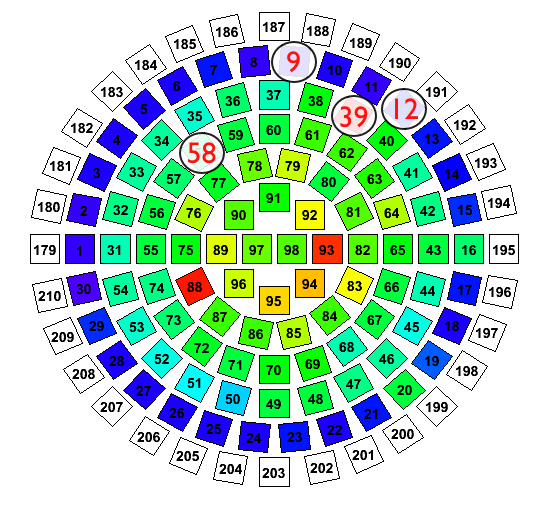
\includegraphics[width=0.4\linewidth]{plots/NN/TopLightPattern_withDeadPMTs.png}
\caption[Simulated light pattern for the top PMT array, with indicated not working channels]{Simulated light pattern for the top PMT array, with indicated not working channels.\\ \\}
\label{figLightPattern}
%\end{figure}
\end{floatingfigure}

\begin{equation}
\Delta\omega_{ij} = \eta\ \delta_{j}\ o_{i},
\end{equation}
where 
\begin{equation}
\nonumber
\delta_{j} = 
\left\{\begin{matrix}
f_{j}(net_{j})(t_{j}-o_{j})\ \text{if {\it j} is an output unit} \\
f_{j}(net_{j})\sum_{k}\delta_{k}\omega_{jk}\ \text{if {\it j} is a hidden unit}
\end{matrix}\right.
\end{equation}
and 
$j$ - index of the current unit; 
$i$ - index of the unit which is a predecessor to the current one; 
$k$ - index of the unit which is a successor the current one; 
$\eta$ - learning factor (constant); 
$\omega_{ij}$ - link from the current unit to the preceding unit; 
$\omega_{jk}$ - link from the current unit to the successor unit; 
$t_{j}$ - teaching input (desired output) of the current unit; 
$o_{i}$ - output of the preceding unit; 
$\delta_{j}$ - error, defined as a difference between the real output and the teaching input of the current unit; 
$net_{j}$ - net input in unit $j$; 
$f_{j}$ - activation function of unit $j$.
The input of a network layer is computed by summing up all weighted activations and by applying  the hyperbolic tangent function:
\begin{equation}
\tanh{(x)} = \frac{e^{2x}-1}{e^{2x}+1}.
\end{equation}
Hence, the new activation values are in range [-1,1]. The identity output function computes the output of every unit from current activation of this unit, and makes it possible to process the activation before an output occurs. 
The calculated weights of the links between the units are used for the light pattern recognition and event localization in the XENON100 TPC.
\\


\section{Study of the Reconstruction Performance with Monte Carlo Simulations}
\label{secNNmc}

\begin{figure}[!t]
\centering
\subfigure[]{
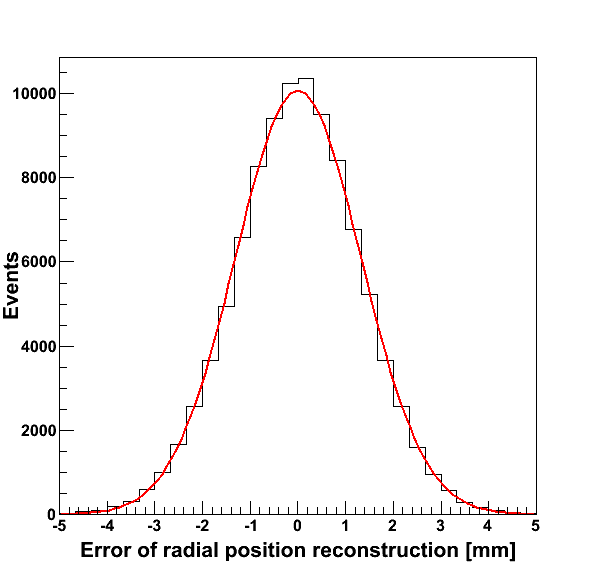
\includegraphics[height=0.4\linewidth]{plots/NN/Rerror.png}
\label{figNNmcRadii_1}}
\subfigure[]{
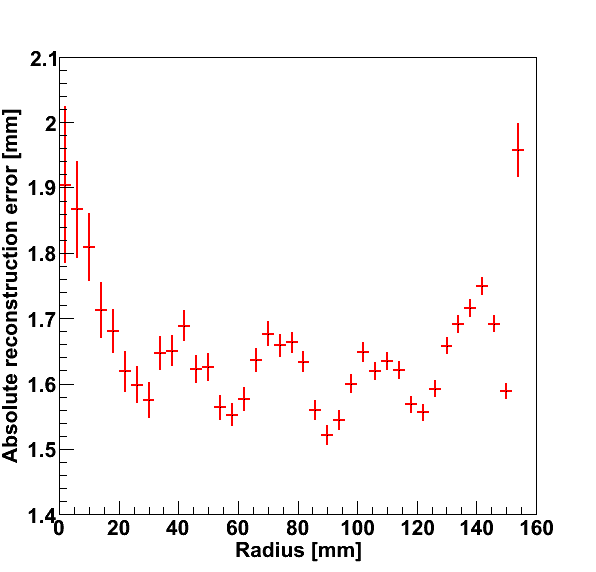
\includegraphics[height=0.4\linewidth]{plots/NN/RerrorAbs_vs_R_correctedAxis.png}
\label{figNNmcRadii_2}}
\caption[Reconstruction of the radial positions with the neural network algorithm on Monte Carlo data]{Reconstruction of the radial positions with NN algorithm on Monte Carlo data: (a) - difference between the simulated and reconstructed radii. The $\sigma$ of the Gaussian fit is 1.3~mm. (b) - absolute reconstruction error (Euclidean distance between the simulated and reconstructed positions) as a function of the target volume radius. The observed behavior is due to the radial arrangement of the top array PMTs, which results in the fluctuation of S2 LCE (see Fig.~\ref{figLCEs2_1}).}
\label{figNNmcRadii}
\end{figure}

\begin{figure}[!b]
\centering
\subfigure[]{
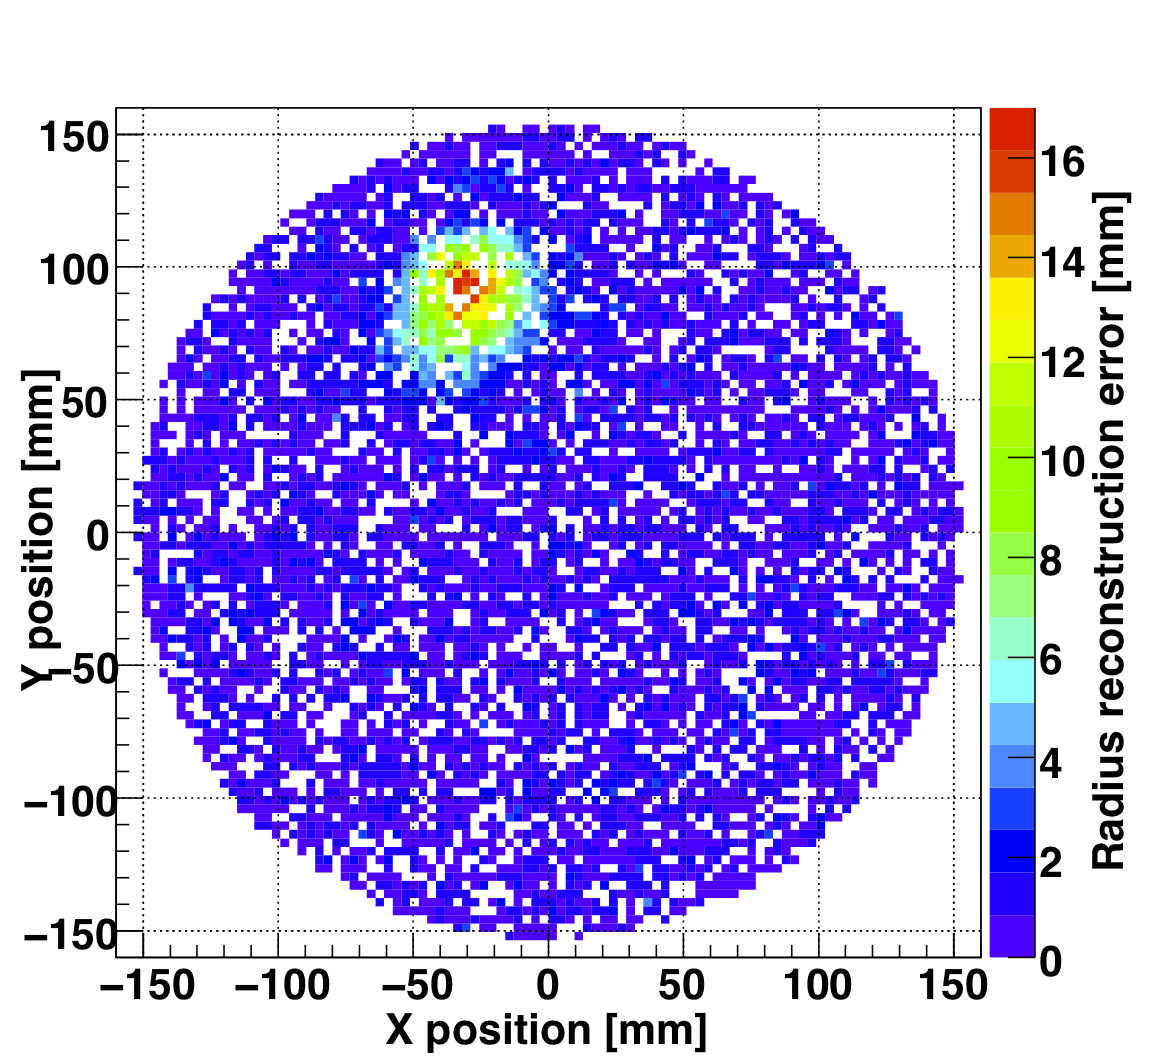
\includegraphics[height=0.385\linewidth]{plots/NN/PosrecMC_1dead_cut.png}
\label{figDeadChannels_1}}
\subfigure[]{
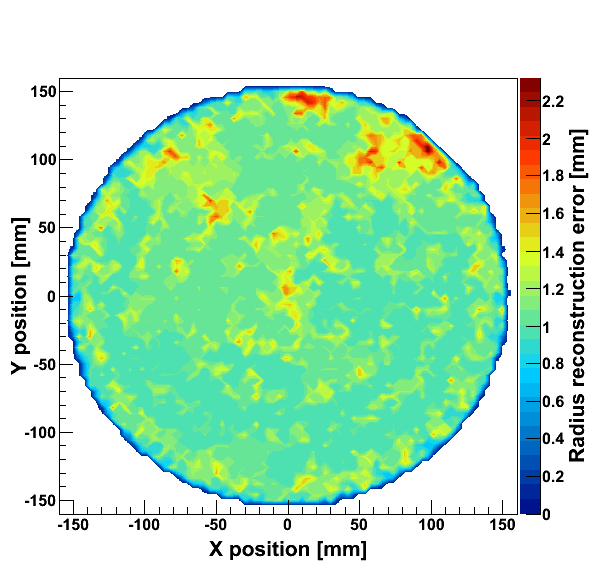
\includegraphics[height=0.4\linewidth]{plots/NN/ReconstructionError_MC_XY.png}
\label{figDeadChannels_2}}
\caption[Training of the reconstruction algorithm for the presence of not working channels]{Training of the reconstruction algorithm for the presence of not working channels: (a) - reconstruction with the original algorithm on a Monte Carlo data with PMT 58 switched off; (b) - Monte Carlo data with 4 not working PMTs and an algorithm trained to account for this.}
\label{figDeadChannels}
\end{figure}

The performance of the NN position reconstruction algorithm has been determined on the patterns that have not been trained during learning. For this purpose, an independent dataset has been generated with a Monte Carlo simulation. Even though the $X$ and $Y$ coordinates of an event are reconstructed with the developed algorithm, the radial coordinate is commonly used in the analysis, i.e. fiducial volume cuts, due to the cylindrical symmetry of the detector. The difference between the simulated and reconstructed radial positions of the events is shown in Fig.~\ref{figNNmcRadii_1}. The distribution is Gaussian and is centered at zero, thus there is no systematic bias in the reconstructed positions. The $\sigma$ spread of the Gaussian fit  characterizes the reconstruction error and is 1.3~mm. The absolute reconstruction error has been defined as the Euclidean distance between the simulated and reconstructed positions in $XY$ plane. The dependence of this parameter on the radial position of the events is shown in Fig.~\ref{figNNmcRadii_2}. The reconstruction uncertainty is not constant with radius due to the concentric arrangement of the PMTs in the top array, and is larger near the center and at the edge of the target volume due to lower PMT coverage in these regions (Fig.~\ref{figPMTarrangement_1}). 


%\begin{floatingfigure}[l]{0.4\textwidth}
%\begin{figure}[!h]
%\centering
%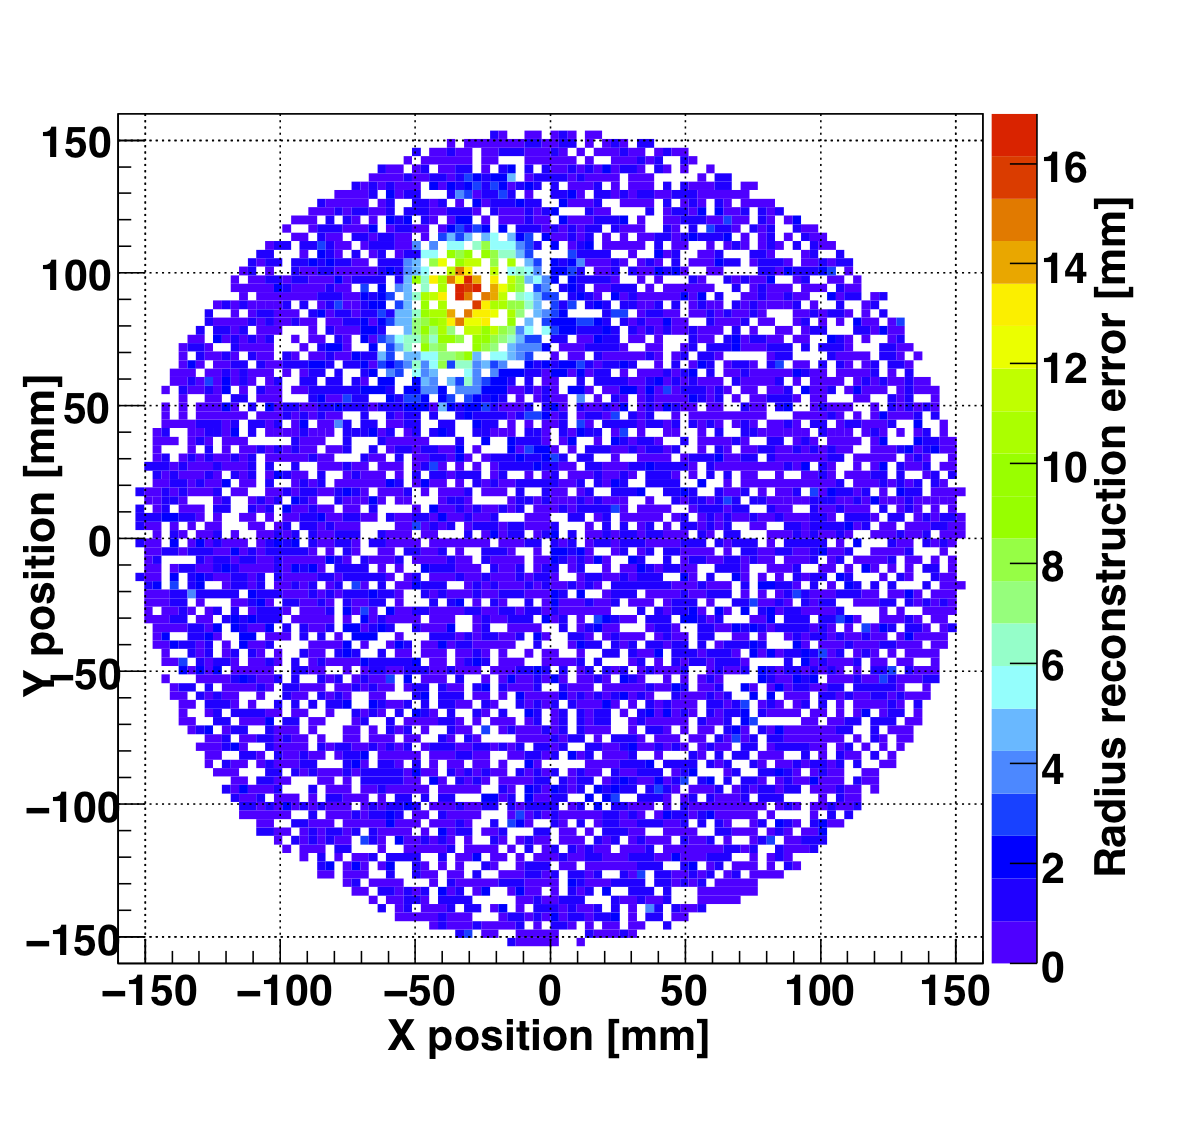
\includegraphics[height=0.2\linewidth]{plots/NN/PosrecMC_1dead.png}
%\caption{Reconstruction with the original algorithm on Monte Carlo data with PMT 58 switched off.}
%\label{figDeadPMT}
%\end{figure}
%\end{floatingfigure}

The performance of the position reconstruction is strongly affected if any PMT of the top array is not working during the data acquisition, and the  originally developed algorithm cannot be used. An example of such problem is shown in Fig.~\ref{figDeadChannels_1}, where PMT~58 has been switched off in the simulation, and the original algorithm has been used for reconstruction of the event vertex. The uncertainty on reconstructed radius for interactions right under the not working channel is $>$10~mm, an order of magnitude worse than in normal conditions.

As it was mentioned in Section~\ref{secPMT}, 8 PMTs stopped working during the detector operation since it was last opened for maintenance, and 4 of them are located in the top array. In order to correctly reconstruct the event vertex for the data acquired starting with the commissioning run in Fall 2009, these PMTs have to be taken into account in the Monte Carlo simulation that is used to train the algorithm, and the corresponding neurons have to be disconnected from the network. The performance of the NN algorithm, which is trained to account for the 4 not working channels, is shown in Fig.~\ref{figDeadChannels_2}. The radial reconstruction uncertainty is only slightly worse for events right under the broken PMTs, being about 2~mm.


\section{Reconstruction of Event Vertex in the Measured Data}
\label{secNNdata}

\begin{figure}[!b]
\centering
\subfigure[background]{
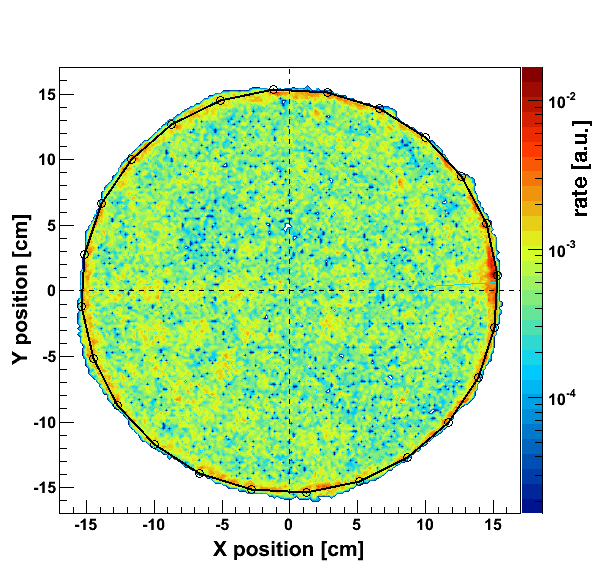
\includegraphics[height=0.4\linewidth]{plots/NN/PosrecBG100keV_withAxis.png}
\label{figPosRecAmBeBG_1}}
\subfigure[$^{241}$Am-Be]{
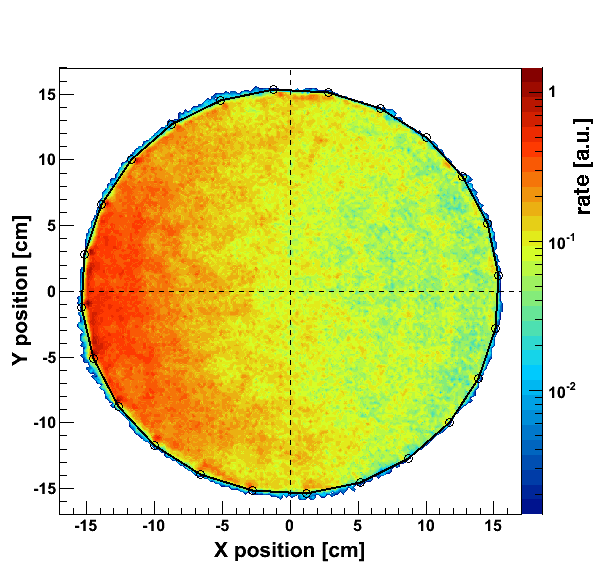
\includegraphics[height=0.4\linewidth]{plots/NN/XYreconstruction_AmBe_withAxis.png}
\label{figPosRecAmBeBG_2}}
\caption[Reconstruction of the event vertex for background and $^{241}$Am-Be data]{Reconstruction of the event vertex for background (a) and $^{241}$Am-Be data using a source outside the TPC (b). The black polygon line shows the physical dimensions of the TPC, representing the 24 interlocking PTFE panels. }
\label{figPosRecAmBeBG}
\end{figure}

The overall performance of the $XY$ vertex reconstruction with the NN algorithm has been tested on the data sets which provide relatively uniform distribution of events within the entire target volume: a background run, and calibration data acquired with an $^{241}$Am-Be neutron source.  In the background data set, events with energies below $\sim$100~keV have been selected. The $^{241}$Am-Be data provides higher statistics in the center of the target volume, as the mean free path of MeV neutrons is much longer than for $\gamma$-rays of smaller or similar energies. 
The $XY$ event vertex reconstructed for both datasets is shown in Fig.~\ref{figPosRecAmBeBG}, together with the physical dimensions of the TPC, which are defined by the 24 interlocking PTFE panels. The excellent resolution of the reconstruction algorithm allows to localize the interlocking points, indicating that the TPC is rotated counterclockwise inside the cryostat by $\sim$4.5$^{\circ}$ in respect to coordinate axes. A small fraction of events lies outside of the polygon, which is within the position reconstruction uncertainty determined on Monte Carlo data. 
A slight clustering pattern in the reconstructed positions can be seen on both plots, which is due to PMT saturation effects for S2s with higher amplitude. A detailed study of this effect is presented in Section~\ref{secPosRecSaturation}.

Of particular interest for the XENON100 experiment is the reconstruction uncertainty at the edge of the target volume, as this impacts the performance of the fiducial volume cuts. The reconstruction has been tested on data acquired with a $^{60}$Co calibration source placed in a copper pipe at different positions around the detector in the middle of the TPC height, by comparison with the data from a GEANT4 based Monte Carlo simulation. In order not to have an impact of PMT non-linearity effects, events with energies $<$100~keV have been selected. The same selection cut has been applied to the simulated data. Radial event distributions of the measured and simulated data are shown in Fig.~\ref{figPosRecCo60_1}, together with the reconstruction with the other two algorithms used in XENON100, $\chi^{2}$ minimization~\cite{Yuan} and SVM regression~\cite{Antonio}. The simulated distribution has been convoluted with the reconstruction uncertainty determined on Monte Carlo data, as described in Section~\ref{secNNmc}. The results obtained with the NN position reconstruction algorithm are in a better agreement with the expectation, compared to performance of $\chi^{2}$-minimization and SVM. However, the reconstructed distribution is slightly biased towards the center of the target volume. This effect is reproduced in the Monte Carlo, when the simulated radial distribution is contracted by 1.03\% (see Fig.~\ref{figPosRecCo60_2}). This might be explained by the combined effect of the higher uncertainty of the NN reconstruction algorithm at large radii, since the outer ring of the PMTs does not fully cover this region, and by the deviation of the electric field close to the field shaping rings. A physical effect due to thermal contraction of the TPC can be excluded at this level. Even though the contraction coefficient of PTFE is rather large (1.5\% when cooled down to the liquid xenon temperature of 182~K)~\cite{PTFEcontraction}, the interlocking panels are fixed by copper rings which do not contract significantly ($<$0.2\% when cooled from room temperature to 182~K)~\cite{CopperContruction}.

\begin{figure}[!h]
\centering
\subfigure[]{
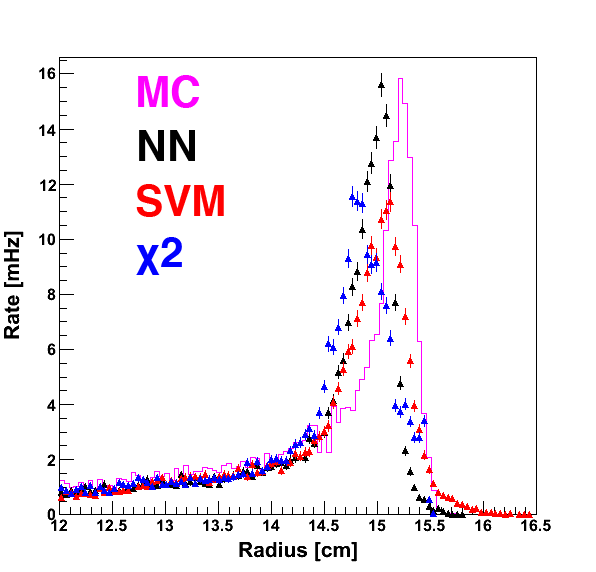
\includegraphics[height=0.4\linewidth]{plots/NN/PosrecCo60_noContraction_withLabels.png}
\label{figPosRecCo60_1}}
\subfigure[]{
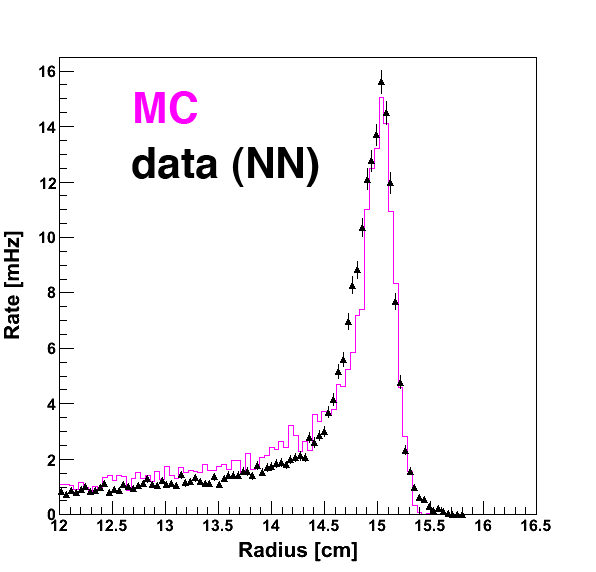
\includegraphics[height=0.4\linewidth]{plots/NN/PosrecCo60_contraction103_withLabels.png}
\label{figPosRecCo60_2}}
\caption[Position reconstruction with the NN, $\chi^{2}$ and SVM algorithms for $^{60}$Co data, and the simulated distribution]{Position reconstruction with the NN (black points), $\chi^{2}$ (blue) and SVM (red) algorithms for $^{60}$Co data, and the simulated distribution (magenta): (a) - only the reconstruction uncertainty determined on Monte Carlo data has been taken into account for the simulation; (b) - simulation includes the contraction of the radial distribution by 1.03\%.}
\label{figPosRecCo60}
\end{figure}

The reconstruction of the radial positions has been also tested with a $^{57}$Co source in a lead collimator placed on top of the cryostat. The length of the collimator was 10~cm, and the diameter of the collimator opening was 2~mm. The distance from the collimator to the liquid surface was $\sim$30~cm. Since the 122~keV $\gamma$-rays from the source have a very low mean free path in liquid xenon ($<$1~cm), the measurements have been performed with a lower amount of xenon in the cryostat, not covering the top veto volume.

The collimator with the positioning device on the top of the cryostat is shown in Fig.~\ref{figPosRecCollimator_1}. The measurements have been performed in the 1st and the 3rd quadrants of the detector volume. The precision of the measurement of the collimator positioning is 1~mm. Taking into account the size of the collimator opening, this corresponds to an uncertainty of $\pm$3~mm on the $\gamma$-beam position at the liquid surface. 

The results of the measurements are shown in Fig.~\ref{figPosRecCollimator_2}. The reconstructed radial positions are in a good agreement with the expectation, and the measured error is $<$2.8~mm, similar to the uncertainty of the set collimator position. A slight (but not significant) deviation in the 1st quadrant has been observed at large radii, this can be explained by not working PMT channels (12 and 39, Fig.~\ref{figLightPattern}), located in this region of the detector volume.

\begin{figure}[!h]
\centering
\subfigure[]{
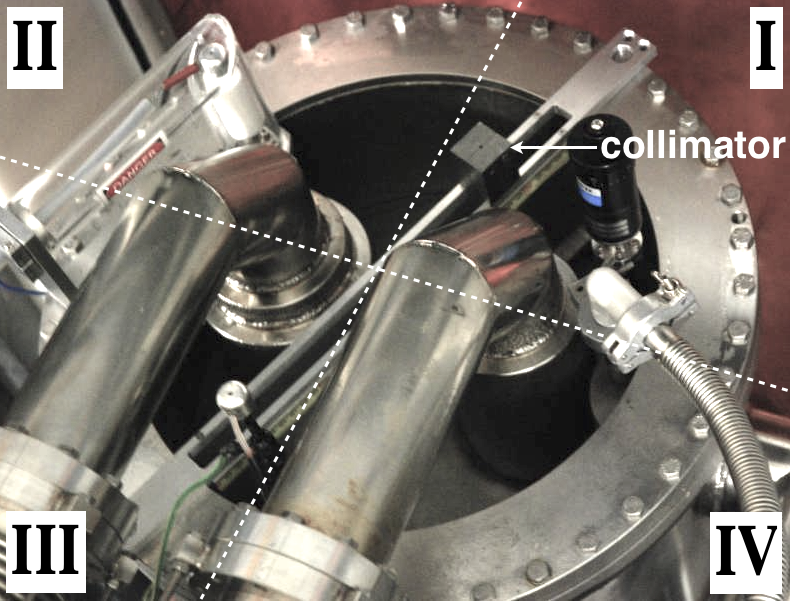
\includegraphics[height=0.37\linewidth]{plots/NN/CollimatorPicture_withLabels3.png}
\label{figPosRecCollimator_1}}
\subfigure[]{
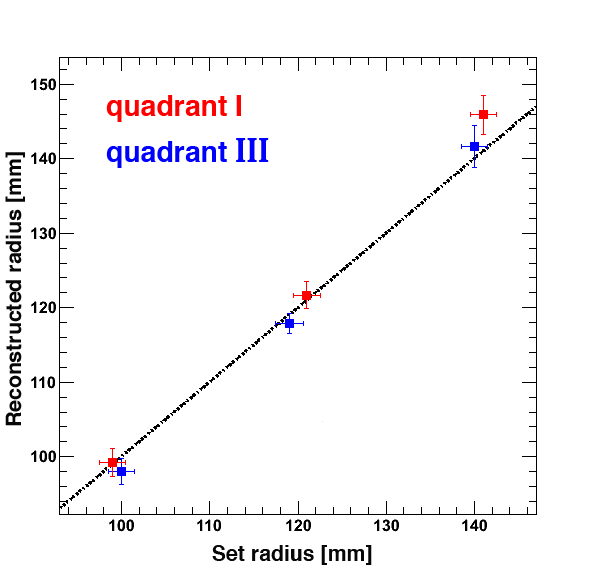
\includegraphics[height=0.4\linewidth]{plots/NN/CollimatorResult_withLabels1.png}
\label{figPosRecCollimator_2}}
\caption[Lead collimator with a $^{57}$Co source on the top of the cryostat, and the results of the test of radial position reconstruction]{Lead collimator with a $^{57}$Co source on the top of the cryostat (a), and the results of the test of radial position reconstruction (b). The dashed line indicates the expectation. Figure published in  Ref.~\cite{xe100-instrument}.}
\label{figPosRecCollimator}
\end{figure}


%source in Fig.\ref{fig:ReconstructionData}. A slight clustering of the events between the PMTs can be seen, which is caused by the PMT saturation for high energy events (no energy cut is used for this plot). 
%The reconstruction performance has been verified on $^{60}$Co calibration data, as shown in Fig.\ref{fig:ReconstructionData} (right). Only events with the energy $<$100 keV are selected. A good agreement is obtained between the measured data and a Monte Carlo simulation. The reconstruction with the algorithms based on $\chi$ minimization and support vector machine regression is also shown on the plot, resulting in worse overall performance than NN method..
%A good resolution of the reconstruction allows to localize the interlocking points of the teflon panels. As it is shown in Fig.\ref{fig:ReconstructionData} (left), the TPC is rotated inside the cryostat by $\sim$4.5$^{\circ}$ in respect to coordinate axes.

%\begin{figure}[!h]
%\begin{center}
%\begin{tabular}{cc}
%\includegraphics[height=0.415\linewidth]{plots/NN/XYreconstruction_AmBe.png}
%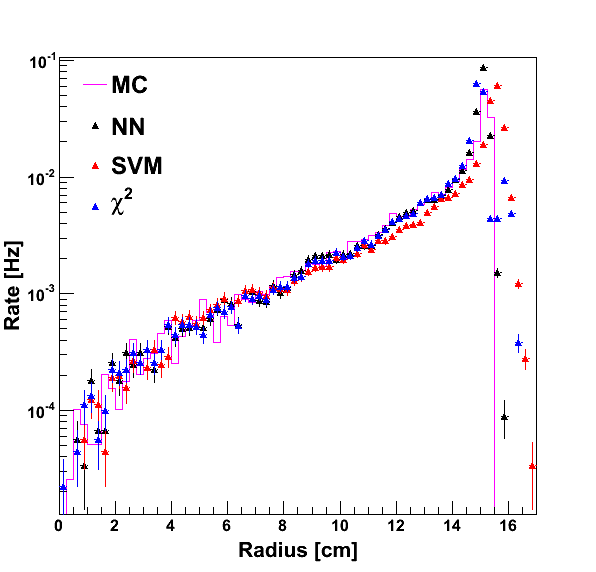
\includegraphics[height=0.407\linewidth]{plots/NN/Rreconstruction_dataMC_log.png}
%\end{tabular}
%\caption{Position reconstruction with NN. {\it Left}: reconstructed {\it xy} positions for Am-Be calibration data (all single scatter events). The polygon represents interlocking teflon panels, which define the outer border of the TPC. The TPC is rotated inside the cryostat by $\sim$4.5$^{\circ}$. {\it Right}: reconstructed radial positions for $^{60}$Co data (events with energy $<$100~keV) and comparison with a MC simulation. The best agreement with MC is provided by the reconstruction algorithm based on NN.}
%\label{fig:ReconstructionData}
%\end{center}
%\end{figure}


